\documentclass[11pt]{report}
\usepackage{fullpage}
%\usepackage{sourcesanspro, sourcecodepro}
\usepackage{minted}
\usepackage{graphicx}
\usepackage{awesomebox}
\usepackage{hyperref}
\usepackage{float} % stops images from moving around
\usepackage[a4paper, total={6in, 8in}, margin=0.75in]{geometry}
\usepackage{etoolbox}
\makeatletter
\patchcmd{\chapter}{\if@openright\cleardoublepage\else\clearpage\fi}{}{}{}
\RequirePackage[T1]{fontenc}
\RequirePackage[default,light,black]{roboto}

% DarkMode
\usepackage{xcolor}
\pagecolor[rgb]{0,0,0} %black
\color[rgb]{0.7,0.7,0.7} %grey

\hypersetup{
    colorlinks=true,
    linkcolor=cyan,
    citecolor=cyan,
    filecolor=cyan,
    urlcolor=cyan,
    pdfborder={0 0 0}
}

\graphicspath{{./images/}}

\title{APSC 258: Lab 1 Manual}
\author{Andre Cox \\ Scott Halston}

\begin{document}
    \maketitle
    \tableofcontents

    \clearpage

    \chapter{Introduction}

    \section{Authors Note}
    The lab manuals are written in a way that not only guides you through the lab but also provides you with exciting examples of how we can apply the concepts learned to real-world problems that you may encounter in your engineering career. For the best learning experience, reading the lab manuals before starting the lab is recommended.
    It is important to note that often, there will not be only one correct answer to a problem. There may be many different solutions that satisfy the problems given in this course's lab reports. Many of the labs for this course will require some trial and error; don't be discouraged if you do not succeed on your first attempt.


    \section{Background}
    Engineers often design complex systems that require a large amount of time and effort to build. Some examples of this that are relative to the content of this course are speech recognition, medical diagnostics, and self-driving cars.
    Making a computer complete any of these tasks may seem near-impossible; luckily for us, we have the power of machine learning to help us solve these problems. In recent times, machine learning has become easily accessible to engineers and researchers, so in the following labs we will set out to create our own machine learning models to create a simple, self-driving car.
    Although our models will be relatively simple, the techniques you will learn can be applied to every engineering discipline to solve complex problems.


    \section{Introducing the Self Driving Car Project}
    Over the course of this semester, we will be creating a rudimentary self-driving car. As it is impractical, and unsafe, for us to train a typical car to drive around in the real world, we will instead use remote-controlled cars. This car will have a camera that can see the "road" which we will create using painter's tape. At the end of the semester, we will have a competition to see how capable each team's car is.

    % page break
    \clearpage

    \chapter{Start of the Lab}

    \section{Introducing the Pi Car}
    When you come to your first lab your lab group will be given a remote-controlled car with a computer built right in (PiCarV)! 

    % show image
    \begin{figure}[h]
        \centering
        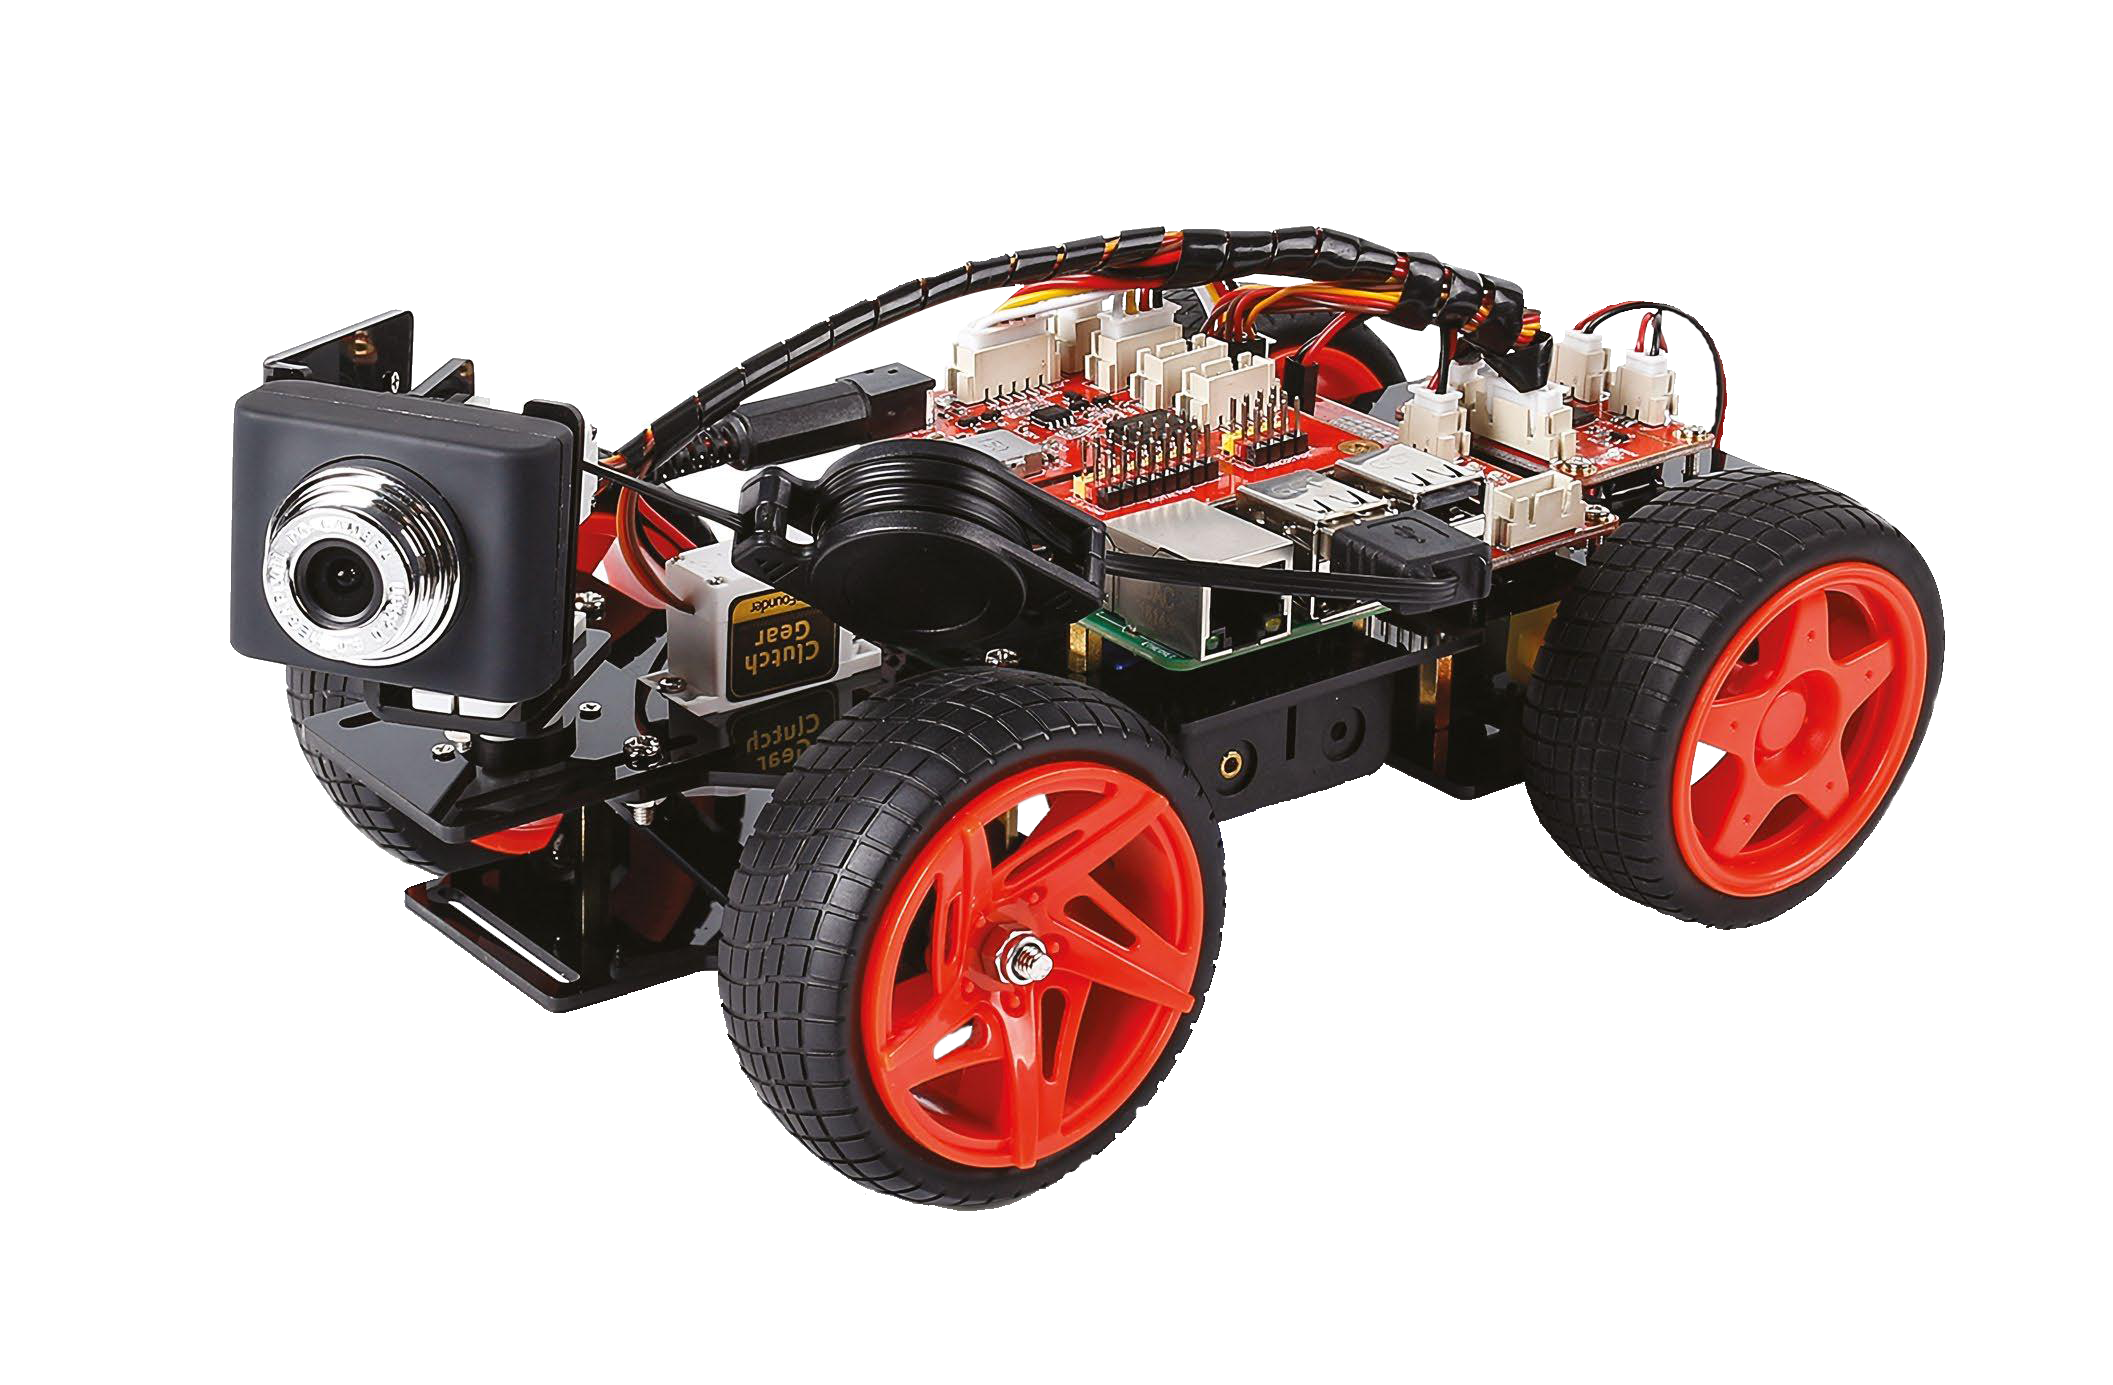
\includegraphics[width=0.8\textwidth]{picarv.png}
        \caption{The Assembled PiCarV}
        \label{fig:The Assembled PiCarV}
    \end{figure}

    The first task is to check if you have received all the components. The PiCarV should already be assembled and ready to go. Make sure you have these components:

    \begin{itemize}
        \item 18650 Lithium-Ion Battery x2 (They should be wrapped in plastic, do not remove this!)
        \item 18650 Charger x1
        \item 18650 Charger Cable x1
    \end{itemize}

    In addition to verifying that you have all received all of the above components, you should look to make sure that nothing is obviously broken and that no cables are unplugged on your PiCarV.

\begin {figure}[h]
    \centering
    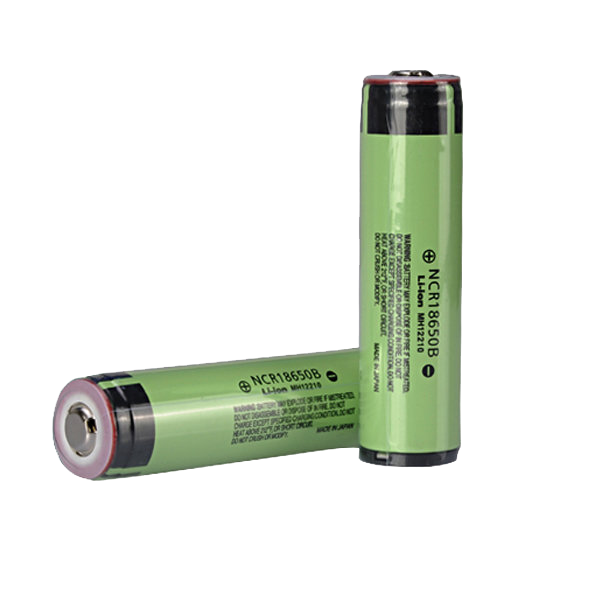
\includegraphics[width=0.5\textwidth]{battery.png}
    \caption{18650 Battery}
    \label{fig: 18650 Battery}
\end{figure}
    
\notebox{
    \textbf{18650 Facts:}
    The 18650 Battery Cell is one of the most common battery cells in the world. They are used in almost every electric car and bike. They can be connected together in series and parallel to create any battery pack an engineer may need. From a small 2-cell battery pack, like in our PiCarV, to a full-size electric car with over 8000 cells.
}

\section{Testing the PiCarV}
To test the PiCarV you will first need to charge the batteries by placing them in the charger. Your charger has 2 buttons on the front, you do not need to touch these.

\cautionbox{
    \textbf{Warning Fire Hazzard:}
    While 18650 batteries are generally very safe, under the wrong circumstances they can be a fire hazard. To alleviate this you should always be present when charging the batteries and make sure you store the batteries away from flammable materials. Store the batteries in room temperature/cool conditions; for instance, do not leave the batteries in a hot car.
}

Once the charger has finished, the batteries can be placed into the PiCarV. Once the batteries are installed, switch on the PiCarV. You should see the lights on the side of the PiCarV start to blink. You can verify that everything is working by opening your Wi-Fi settings on your phone or laptop and checking if a hotspot has been created. The hotspot network should be called PiCarV followed by a string of letters and numbers. Make a note of the name of this network because, when multiple PiCars are running simultaneously, it may be difficult to determine which network belongs to which PiCar.

\section{Connecting the controller to the PiCarV}
We provide a simple controller app that you can use to check that your PiCarV is working. You can download the app from the following link. 
% include hyperlink
\href{https://github.com/PiCarV/Controller/releases}{PiCar Controller} Make sure you get the correct version for your operating system. EXE for windows and DMG for mac.


Once you have installed the controller you can connect your computer to the PiCar hotspot the password is "raspberry". Next, you can open the controller app and enter the IP address of the PiCarV in the top right corner. The IP address is "192.168.0.10". Once this is entered the text that says "connected: false" should change to "connected: true" and you should see a live stream from the camera. Try to have a go controlling the PiCarV with either WASD or the arrow keys. 

% show image
\begin{figure}[h]
    \centering
    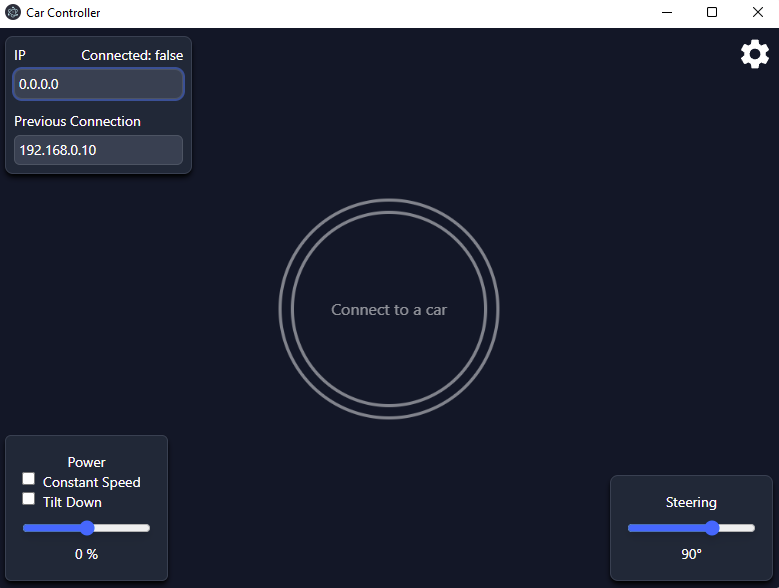
\includegraphics[width=0.8\textwidth]{controller.png}
    \caption{Controller}
    \label{fig:Controller}
\end{figure}

\chapter{Finishing Up}
Now we can control the PiCar through a simple application. The PiCar is ready for your next lab where you will learn how to send your own commands to run the PiCar using Python.

\end{document}




